\batchmode
\makeatletter
\def\input@path{{/Users/Adam/Dropbox/Stat215A-2013/Labs/Lab2/Lab//}}
\makeatother
\documentclass[english]{article}\usepackage{graphicx, color}
%% maxwidth is the original width if it is less than linewidth
%% otherwise use linewidth (to make sure the graphics do not exceed the margin)
\makeatletter
\def\maxwidth{ %
  \ifdim\Gin@nat@width>\linewidth
    \linewidth
  \else
    \Gin@nat@width
  \fi
}
\makeatother

\IfFileExists{upquote.sty}{\usepackage{upquote}}{}
\definecolor{fgcolor}{rgb}{0.2, 0.2, 0.2}
\newcommand{\hlnumber}[1]{\textcolor[rgb]{0,0,0}{#1}}%
\newcommand{\hlfunctioncall}[1]{\textcolor[rgb]{0.501960784313725,0,0.329411764705882}{\textbf{#1}}}%
\newcommand{\hlstring}[1]{\textcolor[rgb]{0.6,0.6,1}{#1}}%
\newcommand{\hlkeyword}[1]{\textcolor[rgb]{0,0,0}{\textbf{#1}}}%
\newcommand{\hlargument}[1]{\textcolor[rgb]{0.690196078431373,0.250980392156863,0.0196078431372549}{#1}}%
\newcommand{\hlcomment}[1]{\textcolor[rgb]{0.180392156862745,0.6,0.341176470588235}{#1}}%
\newcommand{\hlroxygencomment}[1]{\textcolor[rgb]{0.43921568627451,0.47843137254902,0.701960784313725}{#1}}%
\newcommand{\hlformalargs}[1]{\textcolor[rgb]{0.690196078431373,0.250980392156863,0.0196078431372549}{#1}}%
\newcommand{\hleqformalargs}[1]{\textcolor[rgb]{0.690196078431373,0.250980392156863,0.0196078431372549}{#1}}%
\newcommand{\hlassignement}[1]{\textcolor[rgb]{0,0,0}{\textbf{#1}}}%
\newcommand{\hlpackage}[1]{\textcolor[rgb]{0.588235294117647,0.709803921568627,0.145098039215686}{#1}}%
\newcommand{\hlslot}[1]{\textit{#1}}%
\newcommand{\hlsymbol}[1]{\textcolor[rgb]{0,0,0}{#1}}%
\newcommand{\hlprompt}[1]{\textcolor[rgb]{0.2,0.2,0.2}{#1}}%

\usepackage{framed}
\makeatletter
\newenvironment{kframe}{%
 \def\at@end@of@kframe{}%
 \ifinner\ifhmode%
  \def\at@end@of@kframe{\end{minipage}}%
  \begin{minipage}{\columnwidth}%
 \fi\fi%
 \def\FrameCommand##1{\hskip\@totalleftmargin \hskip-\fboxsep
 \colorbox{shadecolor}{##1}\hskip-\fboxsep
     % There is no \\@totalrightmargin, so:
     \hskip-\linewidth \hskip-\@totalleftmargin \hskip\columnwidth}%
 \MakeFramed {\advance\hsize-\width
   \@totalleftmargin\z@ \linewidth\hsize
   \@setminipage}}%
 {\par\unskip\endMakeFramed%
 \at@end@of@kframe}
\makeatother

\definecolor{shadecolor}{rgb}{.97, .97, .97}
\definecolor{messagecolor}{rgb}{0, 0, 0}
\definecolor{warningcolor}{rgb}{1, 0, 1}
\definecolor{errorcolor}{rgb}{1, 0, 0}
\newenvironment{knitrout}{}{} % an empty environment to be redefined in TeX

\usepackage{alltt}
\usepackage[T1]{fontenc}
\usepackage[latin9]{inputenc}
\usepackage{geometry}
\geometry{verbose,tmargin=1in,bmargin=1in,lmargin=1in,rmargin=1in}
\usepackage{fancyhdr}
\pagestyle{fancy}
\setlength{\parskip}{\smallskipamount}
\setlength{\parindent}{0pt}
\usepackage{amsthm}
\usepackage{amsmath}

\makeatletter

%%%%%%%%%%%%%%%%%%%%%%%%%%%%%% LyX specific LaTeX commands.
\providecommand{\LyX}{L\kern-.1667em\lower.25em\hbox{Y}\kern-.125emX\@}

%%%%%%%%%%%%%%%%%%%%%%%%%%%%%% Textclass specific LaTeX commands.
\numberwithin{equation}{section}
\numberwithin{figure}{section}

\@ifundefined{date}{}{\date{}}
%%%%%%%%%%%%%%%%%%%%%%%%%%%%%% User specified LaTeX commands.
\pagestyle{empty} 

\makeatother

\usepackage{babel}
\begin{document}

\title{Lab 2 - Linguistic Survey\\
Stat 215A}


\author{Jonathan Fischer}
\date{October 7, 2014}

\maketitle


\section{Introduction}

\section{Redwood Data}

\subsection{Temperature Density Estimates via Kernel Smoothing}

\begin{figure}
\begin{center}
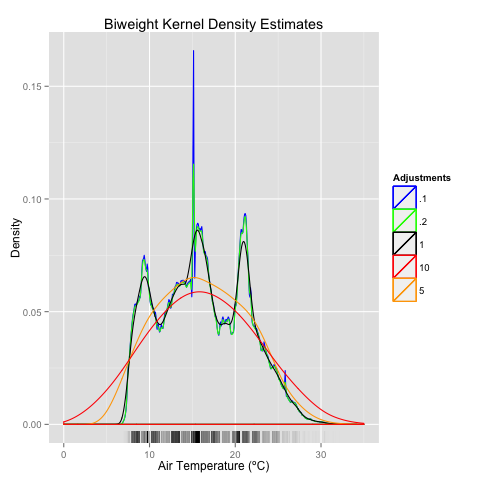
\includegraphics[scale = .4]{Temperature_Density_Biweight_Kernel.png}
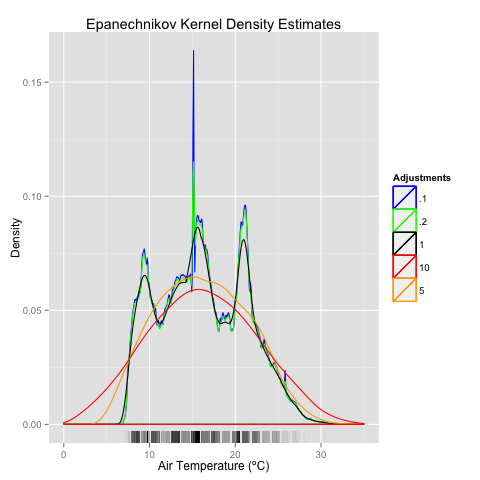
\includegraphics[scale = .4]{Temperature_Density_Epanechnikov_Kernel.png}
\end{center}

\begin{center}
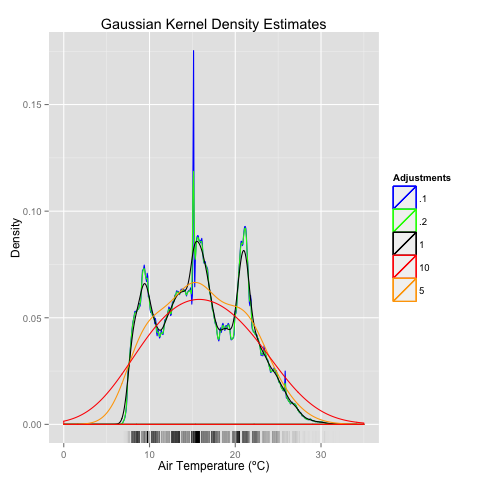
\includegraphics[scale = .4]{Temperature_Density_Guassian_Kernel.png}
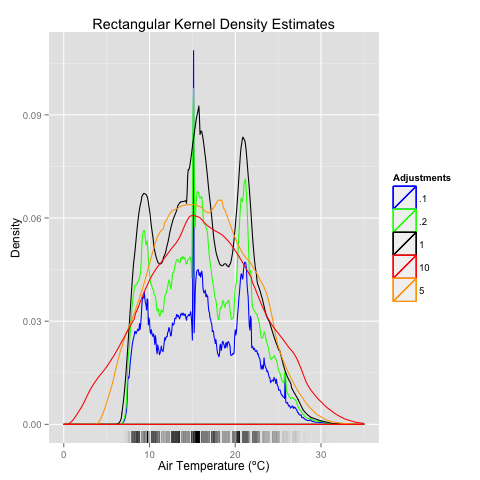
\includegraphics[scale = .4]{Temperature_Density_Rectangular_Kernel.png}
\end{center}
\end{figure}

\subsection{Loess Smoothed Humidity vs Temperature}

\begin{figure}

\begin{center}
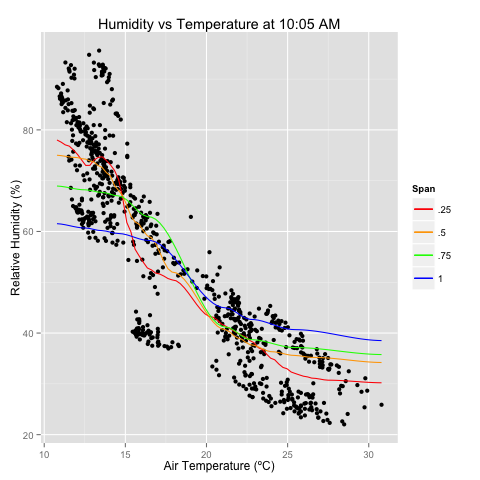
\includegraphics[scale = .4]{Humidity_Temperature_Loess_0.png}
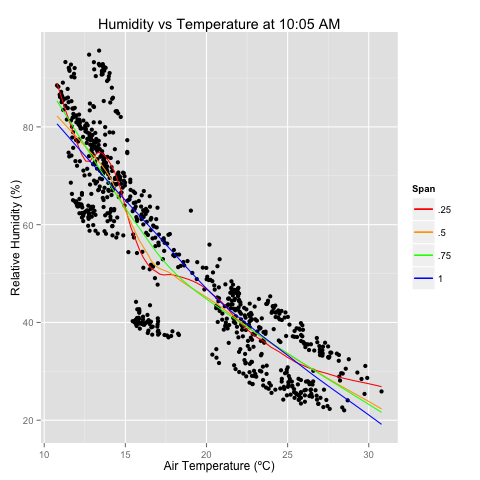
\includegraphics[scale = .4]{Humidity_Temperature_Loess_1.png}
\end{center}

\begin{center}
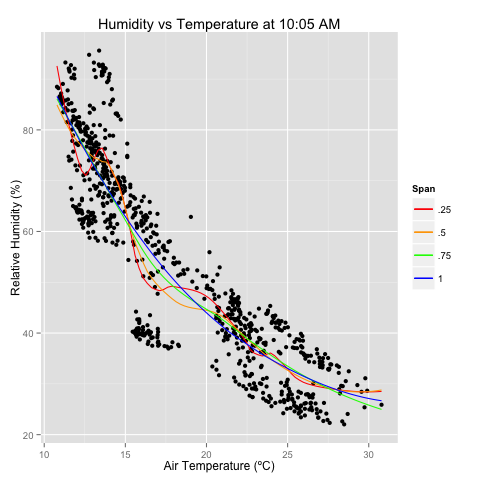
\includegraphics[scale = .4]{Humidity_Temperature_Loess_2.png}
\end{center}
\end{figure}



\section{Linguistic Data}


\subsection{Data quality and cleaning}

This dataset isn't as bad as the redwood data, but there are still
some issues. You should discuss them here and describe your strategies
for dealing with them.


\subsection{Exploratory Data Analysis}

This is where you compare pairs of questions with discussion and plots.


\section{Dimension reduction methods}

This is where you discuss and show plots about the results of whatever
dimension reduction techniques you tried - PCA, hierarchical clustering,
K-means, random projections, etc.


\section{Stability of findings to perturbation}


\section{Conclusion}
\end{document}
